% Asset ID: A22ProjectilesTikZ-003
% Purpose: Diagram for a particle projected horizontally from a height.
\documentclass[tikz,border=8pt]{standalone}
\usepackage{amsmath}
\usetikzlibrary{arrows.meta,calc}
\begin{document}
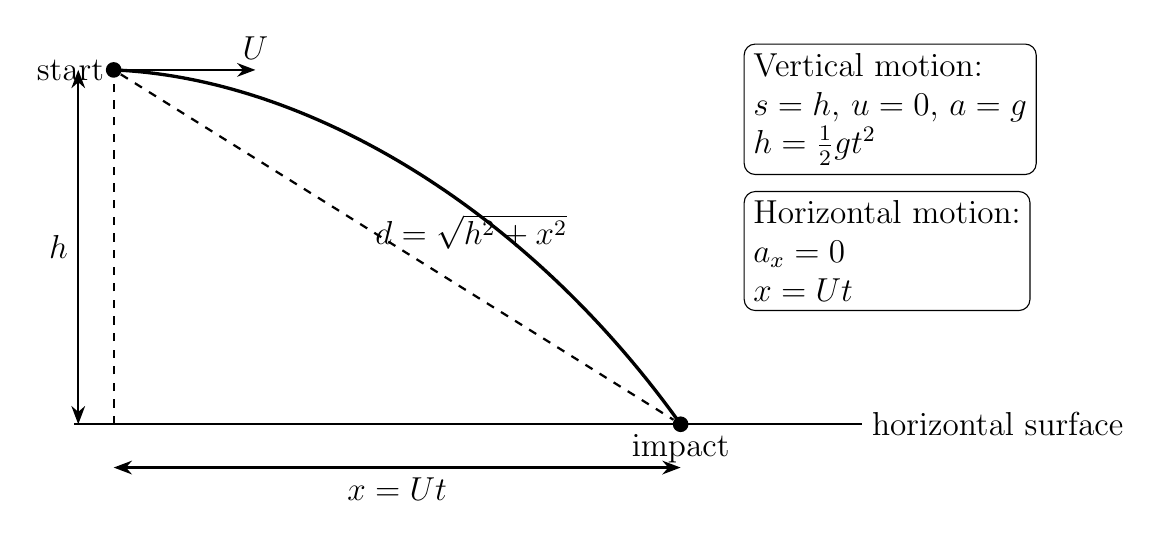
\begin{tikzpicture}[>=Stealth,pathcurve/.style={very thick},arrow/.style={->,thick},guide/.style={dashed,thick},label/.style={font=\large},point/.style={circle,fill=black,inner sep=2pt}]
\draw[thick] (-0.5,0)--(9.5,0) node[right,label]{horizontal surface}; \draw[guide] (0,0)--(0,4.5);
\node[point] (O) at (0,4.5) {}; \node[point] (A) at (7.2,0) {}; \node[left,label] at (O) {start}; \node[below,label] at (A) {impact};
\draw[pathcurve] (0,4.5) .. controls (2.4,4.4) and (5.2,2.8) .. (7.2,0);
\draw[arrow] (O)--++(1.8,0) node[above,label] {$U$};
\draw[<->,thick] (-0.45,0)--(-0.45,4.5) node[midway,left,label] {$h$};
\draw[<->,thick] (0,-0.55)--(7.2,-0.55) node[midway,below,label] {$x=Ut$};
\draw[guide] (O)--(A); \node[above right,label] at (3.2,2.1) {$d=\sqrt{h^2+x^2}$};
\node[draw,rounded corners,align=left,font=\large,anchor=west] at (8.0,4.0) {Vertical motion:\\$s=h$, $u=0$, $a=g$\\$h=\frac12gt^2$};
\node[draw,rounded corners,align=left,font=\large,anchor=west] at (8.0,2.2) {Horizontal motion:\\$a_x=0$\\$x=Ut$};
\end{tikzpicture}
\end{document}
